La arquitectura propuesta para el TFM incluye los siguientes servidores:

\begin{enumerate}
    \item \textbf{Servidor Bacula en Debian}: Este servidor actuará como el Director de Bacula y alojará el Catálogo en una base de datos PostgreSQL.
    \item \textbf{Servidor Debian para Prácticas de Archivos}: Actuará como cliente de Bacula para realizar prácticas de respaldo de archivos.
    \item \textbf{Servidor Debian para Prácticas con Bases de Datos}: Se utilizará para prácticas de respaldo de bases de datos, funcionando como otro cliente de Bacula.
    \item \textbf{Servidor Windows para Prácticas de Archivos}: Este servidor funcionará como cliente en un entorno Windows, demostrando la capacidad de Bacula para trabajar en entornos mixtos.
\end{enumerate}







\begin{figure}[H]
    \centering
    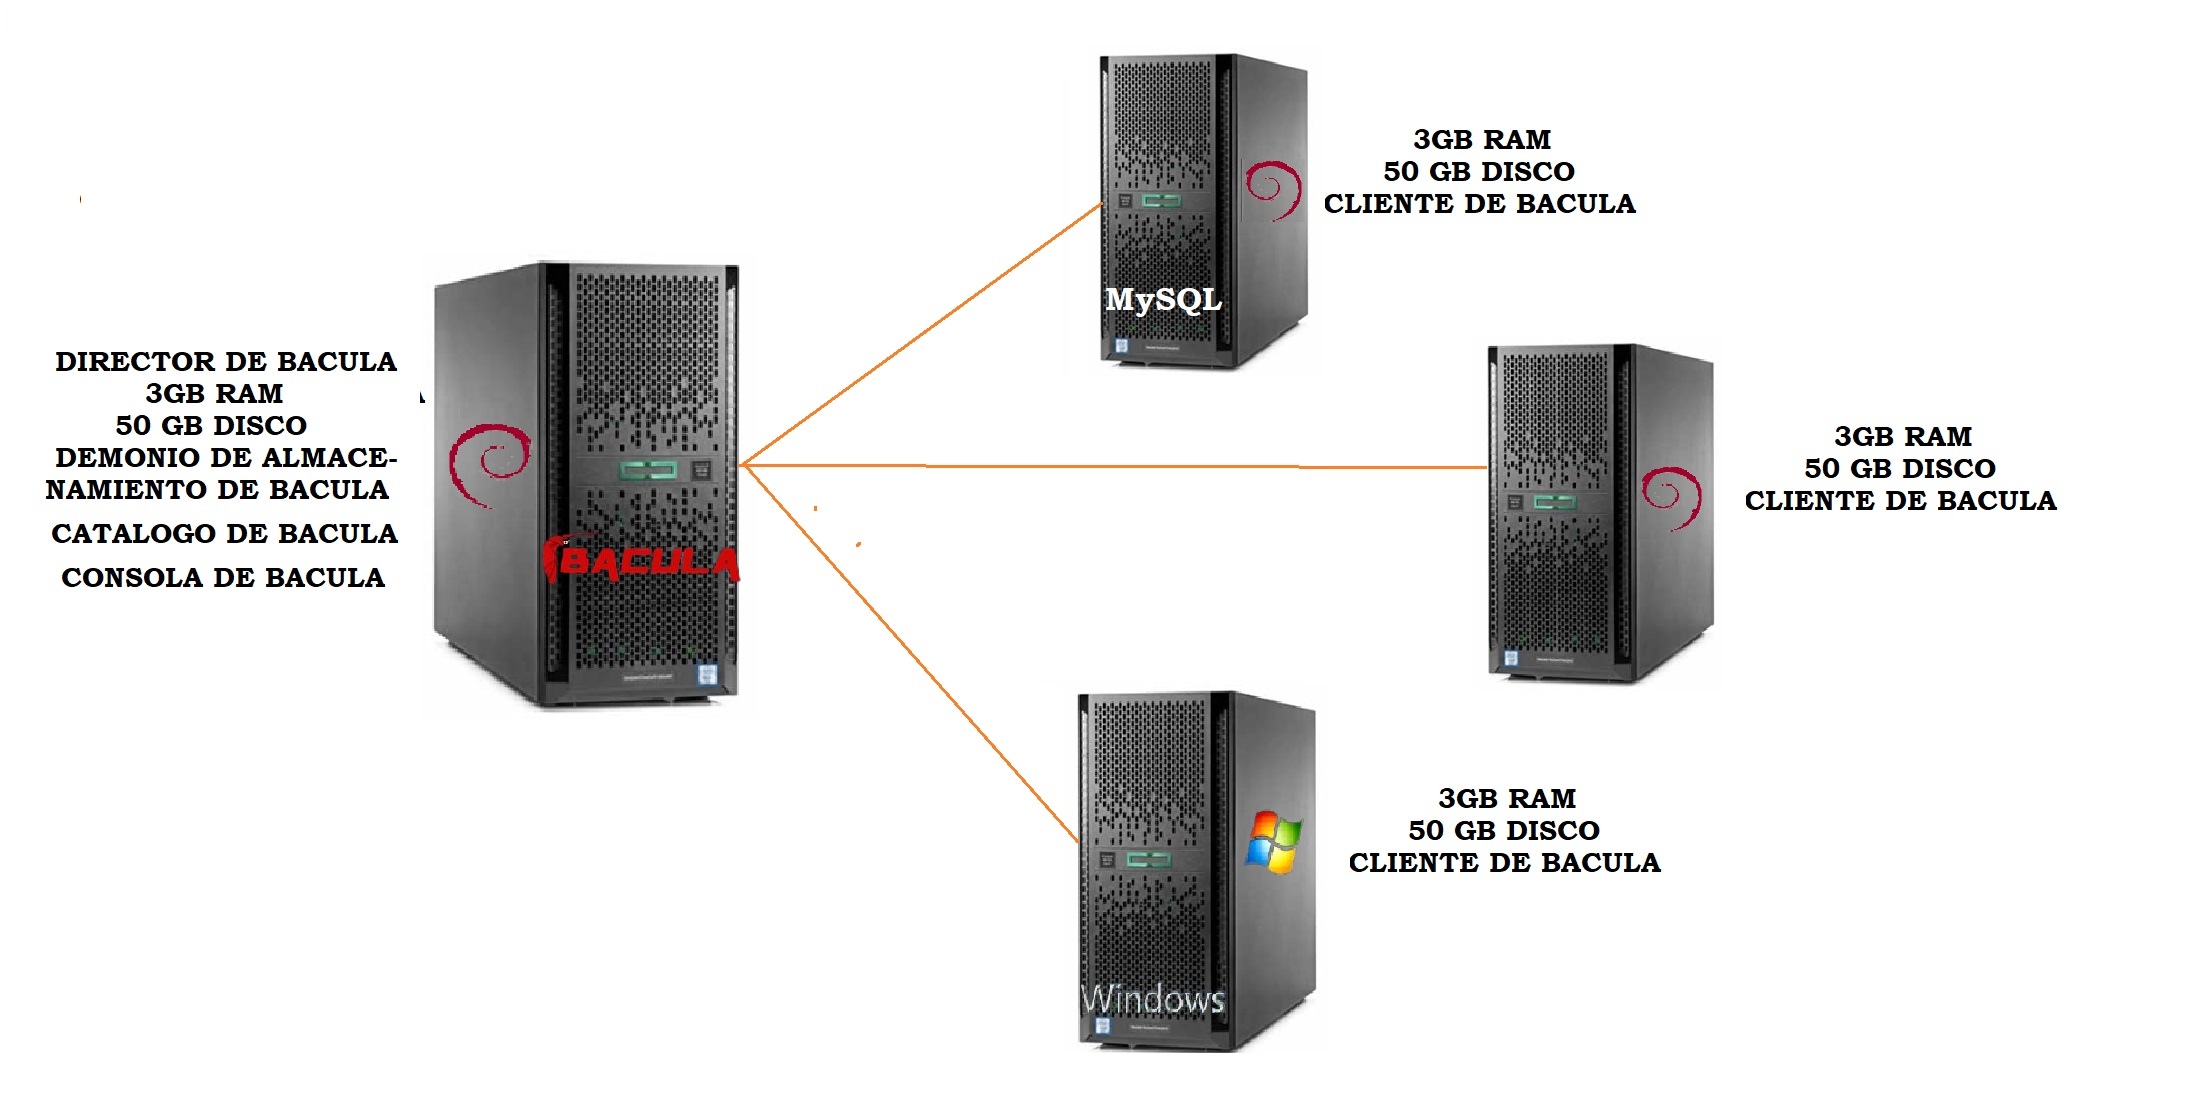
\includegraphics[width=1\textwidth]{imagenes/graficos/BACULA.jpg} % Ajusta el nombre de archivo y la escala según sea necesario
    \caption{Diagrama de la arquitectura de prueba.}
    \label{fig:mi-grafico}
\end{figure}





\subsection{Implementación de los Demonios de Bacula}

La arquitectura de Bacula está diseñada para proporcionar una solución robusta y flexible para la gestión de copias de seguridad en entornos distribuidos. Cada demonio de Bacula juega un papel crítico en este ecosistema, asegurando la eficiencia y seguridad en la realización de backups y restauraciones. A continuación, se describe la implementación de cada demonio dentro de nuestra arquitectura específica.

\subsubsection{Director de Bacula}

El \textbf{Director de Bacula} es el componente central de nuestra arquitectura de backups, encargado de coordinar todas las operaciones de backup y restauración. Este demonio está configurado en nuestro \textit{servidor Debian principal}, el cual actúa como el cerebro del sistema de backups, gestionando tanto la lógica de las operaciones como las políticas y programaciones de los backups.

\begin{itemize}
    \item \textbf{Ubicación:} Servidor Debian principal.
\end{itemize}

\subsubsection{Demonio de Almacenamiento de Bacula}

El \textbf{Demonio de Almacenamiento de Bacula} gestiona los dispositivos físicos o virtuales donde se almacenan los backups. Para optimizar el rendimiento y la escalabilidad de nuestro sistema, este demonio se implementa tanto en el servidor Debian principal como en un \textit{servidor de almacenamiento dedicado}, proporcionando así redundancia y flexibilidad en las opciones de almacenamiento.

\begin{itemize}
    \item \textbf{Ubicaciones:} Servidor Debian principal y servidor de almacenamiento dedicado.
\end{itemize}

\subsubsection{Catálogo de Bacula}

El \textbf{Catálogo de Bacula}, implementado usando \textit{PostgreSQL}, ofrece un índice detallado y metadatos de todas las copias de seguridad y restauraciones realizadas. Este componente es crucial para la gestión eficiente de los backups, permitiendo búsquedas rápidas y la administración de los datos almacenados. El Catálogo se aloja en el \textit{servidor Debian principal}, junto al Director de Bacula, para facilitar la comunicación y el acceso a los datos.

\begin{itemize}
    \item \textbf{Ubicación:} Servidor Debian principal, con PostgreSQL como sistema de gestión de base de datos.
\end{itemize}

\subsubsection{Consola de Bacula}

La \textbf{Consola de Bacula} proporciona la interfaz de usuario para la gestión y monitoreo de las operaciones de backups y restauraciones. Para garantizar un acceso administrativo conveniente, la consola se instala en el \textit{servidor Debian principal} y también está disponible para los administradores a través de sus estaciones de trabajo personales, permitiendo la gestión remota del sistema de backups.

\begin{itemize}
    \item \textbf{Ubicaciones:} Servidor Debian principal y estaciones de trabajo de administradores.
\end{itemize}

\subsubsection{Cliente de Bacula}

El \textbf{Cliente de Bacula} o File Daemon se instala en cada sistema que requiere ser respaldado. En nuestra arquitectura, esto incluye el \textit{servidor Debian para prácticas de archivos}, el \textit{servidor Debian para prácticas con bases de datos}, y el \textit{servidor Windows para prácticas de archivos}. Estos clientes son responsables de enviar los datos al Demonio de Almacenamiento bajo la dirección del Bacula Director.

\begin{itemize}
    \item \textbf{Ubicaciones:} Servidor Debian para prácticas de archivos, servidor Debian para prácticas con bases de datos, y servidor Windows para prácticas de archivos.
\end{itemize}

















\subsection{Tipos de backup}
En la gestión de copias de seguridad con Bacula, como en muchos otros sistemas de backups, se utilizan diferentes estrategias para optimizar el proceso de almacenamiento, reducir el tiempo necesario para realizar las copias de seguridad y facilitar la recuperación de los datos. Estas estrategias se pueden combinar para crear un plan de backups robusto y eficiente. Las cuatro estrategias principales son: completa (full), diferencial, incremental y mixta.

\subsubsection{Completa (Full)}
En una copia de seguridad completa, se copian todos los archivos seleccionados en el sistema. Es la base sobre la cual se realizan las demás estrategias de copia de seguridad, ya que cualquier método de restauración comienza con una copia completa.

\textbf{Escenarios recomendados}: La copia de seguridad completa es ideal para iniciar un ciclo de backups, asegurando que se tenga al menos una versión íntegra de todos los datos. Se recomienda realizar copias de seguridad completas periódicamente, dependiendo del tamaño de los datos y de la capacidad de almacenamiento, por ejemplo, semanalmente o mensualmente.

\subsubsection{Diferencial}
Una copia de seguridad diferencial guarda los cambios realizados desde la última copia de seguridad completa. Cada copia diferencial incluye todos los cambios acumulados desde la última copia completa, lo que significa que su tamaño puede crecer considerablemente con el tiempo hasta que se realiza otra copia completa.

\textbf{Escenarios recomendados}: Esta estrategia es útil cuando se desean minimizar los tiempos de restauración manteniendo un equilibrio con el espacio de almacenamiento utilizado. Es ideal para entornos donde los datos cambian con frecuencia, pero donde realizar una copia completa a menudo no es viable. Se pueden programar copias diferenciales diariamente o semanalmente, según la tasa de cambio de los datos.

\subsubsection{Incremental}
Las copias de seguridad incrementales sólo almacenan los datos que han cambiado desde la última copia de seguridad de cualquier tipo (sea completa, diferencial o incremental). Esto minimiza el tiempo necesario para realizar la copia de seguridad y reduce el espacio de almacenamiento requerido.

\textbf{Escenarios recomendados}: Esta estrategia es excelente para datos que cambian diariamente pero en los que el volumen total de los cambios es relativamente pequeño. Permite realizar copias de seguridad frecuentes, como diarias, con un mínimo impacto en los recursos de almacenamiento y en el rendimiento del sistema.

\subsubsection{Mixta}
La estrategia mixta combina las copias de seguridad completas, diferenciales e incrementales de una manera que mejor se adapte a las necesidades específicas de recuperación y almacenamiento de datos de una organización. Un ejemplo común de una estrategia mixta es realizar una copia completa mensualmente, copias diferenciales semanalmente y copias incrementales diariamente.

\textbf{Escenarios recomendados}: Esta estrategia es ideal para entornos con una gran cantidad de datos y requisitos complejos de recuperación. Permite maximizar la eficiencia del almacenamiento y minimizar los tiempos de restauración ajustando la frecuencia de los diferentes tipos de copias de seguridad según las necesidades específicas y la dinámica de cambios de los datos.

\subsubsection{Implementación de Estrategias de Backups en Bacula}

Para evaluar exhaustivamente las capacidades de Bacula en la gestión de copias de seguridad, se implementarán y probarán cuatro estrategias principales: completa, diferencial, incremental y mixta. La finalidad es determinar la eficacia, eficiencia y aplicabilidad de cada estrategia en distintos escenarios. A continuación, se detalla el proceso de implementación y evaluación para cada estrategia de backup.


\textbf{Backup Completo}

Inicialmente, se realizará un backup completo de todos los datos en los servidores configurados. Este paso es fundamental, ya que establece la base sobre la cual se construirán las demás estrategias de backups.

\begin{enumerate}
    \item Ejecución de la copia de seguridad completa en cada servidor para capturar todos los datos existentes.
    \item Documentación del tiempo requerido y del espacio de almacenamiento consumido por esta operación.
    \item Análisis de la eficiencia del proceso de backup completo en términos de duración y uso del almacenamiento.
\end{enumerate}

\textbf{Backup Diferencial
}
Posteriormente, se implementará la estrategia de backup diferencial para entender cómo afecta la acumulación de cambios desde el último backup completo.

\begin{enumerate}
    \item Modificación de una parte significativa de los datos para simular la actividad regular.
    \item Realización de backups diferenciales para capturar los cambios desde el último backup completo.
    \item Evaluación del incremento en tiempo y almacenamiento en comparación con el backup completo.
\end{enumerate}

\textbf{Backup Incremental}
La estrategia de backup incremental se probará para observar su eficiencia en el manejo de cambios diarios mínimos.

\begin{enumerate}
    \item Introducción de cambios adicionales en los datos después del último backup (completo o diferencial).
    \item Ejecución de backups incrementales que solo capturan los cambios desde el último backup de cualquier tipo.
    \item Comparación y análisis del desempeño y la optimización del almacenamiento frente a las estrategias anteriores.
\end{enumerate}

\textbf{Estrategia Mixta}

Por último, se diseñará e implementará una estrategia mixta que combine los métodos completo, diferencial e incremental, ajustándolos a un calendario que maximice la eficiencia del almacenamiento y la rapidez en la restauración.

\begin{enumerate}
    \item Diseño de un esquema de backups que incluya backups completos mensuales, backups diferenciales semanales y backups incrementales diarios.
    \item Implementación del esquema durante un período de prueba para evaluar la cobertura y eficiencia.
    \item Documentación exhaustiva de los resultados, incluyendo el rendimiento, la eficiencia del almacenamiento y la facilidad de recuperación.
\end{enumerate}